\documentclass[tikz,border=10pt]{standalone}
\usepackage{amsmath}
\usetikzlibrary{decorations.pathreplacing, calc, angles, quotes}

\begin{document}
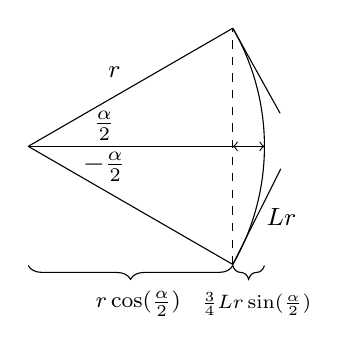
\begin{tikzpicture}[scale=3]

    \def\r{1} 
    \def\angle{60}

    \coordinate (O) at (0,0); 
    \coordinate (A) at (-\angle/2:\r);
    \coordinate (B) at (\angle/2:\r); 
    \coordinate (M) at (0:{\r*cos(\angle/2)});
    \coordinate (N) at (0:\r);

    \draw (A) arc (-\angle/2:\angle/2:\r);

    \draw (O) -- (A);
    \draw (O) -- (B) node[midway, above left, font=\small] {$r$};
    \draw (O) -- (M);
    \draw[dashed] (A) -- (B);
    \draw[<->] (M) -- (N);


    \draw (A) -- +($0.4*({cos(\angle/2+35.9)+0.1},{sin(\angle/2+35.9)+0.1})$) node[midway, right, font=\small] {$Lr$};
    \draw (B) -- +($0.4*({cos(\angle/2+23.1)-0.1},{-sin(\angle/2+23.1)-0.1})$);

    \node at (\angle/4:\r/3) {$\frac{\alpha}{2}$};
    \node at (-\angle/4:\r/3) {$-\frac{\alpha}{2}$};

    \draw[decorate, xshift=-2pt, decoration={brace,amplitude=5pt,mirror,raise=10ex}] 
      ($(O)$) -- ($(M)$) 
      node [black,midway, xshift=0.1cm, yshift=-2cm] 
      {\footnotesize $r\cos(\frac{\alpha}{2})$};

    \draw[decorate, decoration={brace, amplitude=5pt, mirror, raise=10ex}]
        ($(M)$) -- ($(N)$) 
        node [black, midway, xshift=0.1cm, yshift=-2cm, font=\scriptsize] 
        {$\frac{3}{4}Lr\sin(\frac{\alpha}{2})$};
\end{tikzpicture}
\end{document}
